\chapter{Introduction}\label{intro}

This dissertation describes the development and preliminary implementation of an FPGA-based (field-programmable gate array) readout system for a novel detector technology known as the microwave kinetic inductance detector (MKID, or KID) \citep{day2003broadband, mazin2005microwave}. MKIDs are superconducting resonators which change their resonant frequency in response to the absorption of incident photons that have enough energy to break apart superconducting Cooper pairs. The change in resonant frequency is proportional to the amount of optical power which has been absorbed by the inductor.

The combination of the detector arrays and readout system form the core of a very powerful astronomical camera. Although many MKID archictures exist, the one which is primarily discussed in this document is the lumped-element kinetic inductance detector (LEKID) \citep{doyle2008lumped}. The tunable resonant frequencies of MKIDs allow them to be frequency domain multiplexed (FDM) on a single feedline. Current multiplexing factors are in the kilopixel regime. However, the demands of next generation submillimeter (sub-mm) and millimeter-wave (mm-wave) observatories (e.g., CMB-S4 \cite{abitbol2017cmb}) are rapidly pushing the requirements into the megapixel regime. Recent advances in FPGA-based electronics have enabled the use of high speed digital signal processing (DSP) algorithms which are required to match the high multiplexing factors of the detector arrays.

The ASU LEKID readout incorporates firmware, software and electronics which are specifically designed to work with astronomical MKID instruments observing in the sub-mm/mm-wave and far-infrared (FIR) (see Section~\ref{submillimeter}). These instruments are installed at ground-based and stratospheric-balloon-based sub-mm/mm-wave observatories. Although the ASU detector readout has been integrated into several current and planned instruments, it was primarily designed for NASA's Next Generation Balloon-Borne Large Aperture Submillimeter Telescope (BLAST-TNG) \citep{dober}. It's design architecture and initial performance are described in \citet{gordon2016}.

BLAST-TNG (see Section~\ref{blast}) is scheduled for a 28~day balloon-flight from NASA's Long Duration Balloon Facility (LDB) in Antarctica, in winter 2018/2019. It will be the second flight for an MKID-based camera and readout electronics. In July, 2018, the readout system flew on the Italian Space Agency's (ISA) OLIMPO balloon, which was the first test of these emerging technologies in a space-like environment \citep{masi2019kinetic}. The lessons learned from each successive application of the system lead to improvements in system performance and reliability. Successful balloon flights can advance the NASA technology-readiness-level\footnote{\url{https://www.nasa.gov}} of the system to the point at which it can be used on a space-based observatory.

\section{Submillimeter and Millimeter Wave Astronomy}\label{submillimeter}

The primary purpose of the detector technology which is the subject of this dissertation is to enable sub-mm/FIR and mm-wave astronomy. The terminology used to refer to these region of the electromagnetic spectrum is sometimes the source of confusion. In this work, the terms mean the following:

\vspace{5mm}

\textit{Submillimeter}: Wavelengths of 0.1--1~mm (frequencies of 3--0.3~THz, which some astronomers refer to as the terahertz band).

\vspace{5mm}

\textit{Millimeter}: Wavelengths of 1--10~mm (frequencies of 30--300~GHz). The microwave band, here defined as 0.3--300~GHz, overlaps the entire mm-wave band).

\vspace{5mm}

\textit{Far-infrared}: Wavelengths of 25--350~$\upmu$m (frequencies of 12--0.857~THz). FIR shares some overlap with the sub-mm band.

\subsection{Atmospheric Transmission}

The sub-mm/FIR/mm-wave radiation which is detected from space is the heat which is emitted by microscopic particles that fill the spiral arms of galaxies. These particles are collectively called cosmic dust. Since its discovery in the 1930s-40s, the study of the cosmic dust has advanced at a constant but relatively slow pace when compared to other areas of study within astronomy and astrophysics. This lag in development can be attributed to two main factors.

The first factor is that the photons emitted by the dust, which is mostly at temperatures $\leq$100~K, are at very low energy. They therefore require extremely low backgrounds, along with the use of very sensitive devices, such as superconductors, to be detected. The second factor, which is out of the control of humans, is that the troposphere is mostly opaque to the dust emission, due to absorption by water vapor, oxygen and carbon dioxide. Observations of the sub-mm emission from space must therefore be conducted from sites that are as high in altitude and as dry (in terms of precipitable water vapor) as possible. At present, the two best sites in the world are the Atacama desert in Chile, and Antarctica.

\subsection{Cosmic Dust}

In the 19th century, the question of why, given a presumably infinite number of stars, the night sky is mostly dark, came to be known as Olbers' Paradox. The commonly known solutions, which have become more nuanced over the course of time, usually cite the confluence of the vastness of space and the finite sped of light\footnote{The speed limit applies to all forms information transfer.}. While these solutions to Olbers' paradox are sufficient explanations, they usually omit an important contributor to the darkness of the night sky, which is cosmic dust.

Cosmic dust consists of particles ranging from the size of individual molecules (e.g., polycyclic aromatic hydrocarbons (PAHs)) to grains of sizes on the order of $\sim$100~$\upmu$m. These particles permeate the interstellar medium (ISM) of galaxies. Their size distribution, composition and material properties are the subject of ongoing study (see, e.g., \citet{andersson2015interstellar,draine2003interstellar}).

Depending on their size, dust grains scatter high energy photons, and absorb optical and near-infrared (O/NIR) photons. The energy they absorb is reemitted in the sub-mm/mm-wave/FIR. As a result, large swathes of the night sky that would otherwise appear bright to our eyes due to high levels of nearby active star formation (e.g., much of the area encompassed by the constellation of Orion) are enshrouded in darkness due to the presence of insterstellar dust.

When the spectral energy distribution of the observable universe is measured, it appears that roughly the same amount of energy is contained in the sub-mm/far-infrared part of the spectrum as is contained in the O/NIR (peaks at $\sim$1 and $\sim$100~$\upmu$m). By comparing measurements of the GOODS-S region of the sky taken by BLAST 2006 at 250, 350 and 500~$\upmu$m with those taken in other wavebands, it was discovered that approximately half of the sub-mm background light can be associated with individual sub-mm galaxies (SMGs) at cosmological redshifts of $1 \leq z \leq 4$ (\citet{devlin2009over,marsden2009blast,pascale2009blast}). This redshift range corresponds to a period in the universe's history when star formation occurred at rates which are many times higher that which is observed in the present day universe.

\subsection{The Lifecycle of Cosmic Dust}

Conceptually, dust may be thought of as smoke. In \textit{Dust in the Galactic Environment} \citep{whittet2002dust}, the author writes:

\say{The term \textit{smoke} was often used to describe these particles in the early literature. \textit{Smoke} implies the product of combustion, whereas \textit{dust} implies finely powdered matter resulting from the abrasion of solids... The former is arguably more appropriate as a description of the particles condensing in a stellar atmosphere, now regarded as an important source of interstellar grains.}\footnote{Italics added.}

Since its discovery, astronomers have learned that interstellar dust is an important thermodynamic and dynamical catalyst in both small and large scale processes related to star formation in galaxies. In MCs, the dust is collisionally coupled to the gas (the gas-to-dust mass ratio is commonly assumed to be $\sim$100.). The grains are also charged, and their surfaces serve as the hosts of molecular hydrogen formation.

The dust is perpetually recycled in the ISM of galaxies. Some of it is produced in stars, condensing into solid form in the cool  photospheres of AGB stars and planetary nebulae. More dust is produced by supernovae. The dust is spread throughout the ISM by the stellar winds produced by OB and AGB stars, and supernovae. Once in the diffuse ISM, it becomes incorporated into molecular clouds (MCs), the birth places of stars, where it cools to temperatures of 10--100~K. The cold dust then finds its way into the protostellar disks that eventually form into planetary systems. The parent star of the planetary system both destroys and creates new dust, and the cycle repeats itself.

\subsection{The Role of Dust as a Tracer of Cosmic Magnetic Fields}

Observed Galactic star formation rates in MCs are far lower than what is expected from a theoretical model that only includes gravitational collapse. Theorists seeking an explanation for what could be slowing the collapse of prestellar cores have settled on two likely culprits, which are supersonic turbulence and magnetic fields (B-fields). Turbulence can prevent the effective dissipation of gravitational energy, while B-fields can provide an additional source of pressure support that slows, or even halts, the gravitational collapse of MCs.

In the 1930s, astronomers discovered that a small fraction of the O/NIR light which is received from stars is linearly polarized (\citet{hall1949observations,hiltner1949polarization}). The correlation between the polarization of starlight and the previously observed phenomenon of interstellar reddening pointed to cosmic dust as the source. Since the O/NIR starlight is linearly polarized, so is the portion of the starlight which was absorbed by interstellar dust and reemitted at sub-mm/FIR wavelengths.

The cause of the linear polarization of thermal dust emission is understood as being to due to the aspherical nature of the grains. Through a complex alignment mechanism, the aspherical dust grains, which are spinning due to interactions with the gas and radiation field, end up having their long axes orthogonal to the local B-field direction. Consequently, the electric field (E-field) of the thermal radiation emitted by the dust is preferentially oriented along the long axis of the grains. Therefore, rotating the measured polarization angle of the E-field by 90 degrees yields the direction of the B-field. The strength of the B-field is difficult to estimate. However, indirect methods, such as the Davis-Chandrasekhar-Fermi method (DCFM) \citep{chandrasekhar1953magnetic}, can sometimes be used to place upper constraints on the field strength (see~\ref{carina}).

The physics of the alignment mechanism which is responsible for aligning the dust grains with the local B-field has been the subject of long debate \citep{andersson2015interstellar}. The most commonly accepted mechanism is described by the radiative alignment torques (RAT) theory \citep{lazarian2007radiative}. In RAT theory, the alignment is facilitated by both the anisotropy of the radiation field and the paramagnetic nature of the dust grains.

\subsection{The Role of Cosmic Dust as a CMB Foreground}

Due to its polarized thermal emission, cosmic dust poses a problem for polarization masurements of the Cosmic Microwave Background (CMB) radiation. It is now known that the polarized emission from diffuse Galactic dust is the dominant CMB foreground at frequencies above 100~GHz \citep{adam2016planck}. Any attempt to detect primordial B-mode polarization in the CMB will be hindered by the dust foreground emission. The solution to this problem is to carefully map the dust polarization in the same regions which are observed by CMB telescopes, over as wide a waveband as possible. The foreground signal can then be cross-correlated with the CMB measurements, and removed.

\section{Technologies for Submillimeter and Millimeter-Wave Astronomy}

Like the charge-coupled device (CCD), the more widespread quantum detector used in astronomical cameras, MKIDs utilize the photoelectric effect. They are incoherent detectors, measuring the total power in the incident electromagentic radiation (photons), but not the phase. In a semiconductor sensor such as a CCD, the energy band gap of $\sim$1~eV restricts their optical response to between $\sim$0.3--1~$\upmu$m. The superconducting band gap is $\mathcal{O}(10^-3)$ smaller than that of a semiconductor. Consequently, MKIDs (and other superconducting detector technologies) can be engineered to detect radiation spanning the range between mm-waves and Gamma-rays.

The high sensitivity of MKIDs and other superconducting detectors requires that they be operated at a temperature which minimizes their thermal device noise (generation-recombination noise, in an MKID), to below the level of the photon-noise in the passband. As a rule of thumb, this temperature should be $\sim$\gls{Tc}/8 \citep{mazin2013arcons}, where \gls{Tc} is the critical temperature of the device. For a typical MKID \gls{Tc} of $\sim$1.5~K, this corresponds to fridge temperatures of 100--300~mK.

To achieve and maintain such low temperatures throughout an astronomical observation is an engineering feat in its own right. In order to shield the detectors from the thermal radiation of the elements within the optical system, such as mirrors, filters and opto-mechanics, it is necessary to cool as much of the optical system as possible (sometimes to as low as $\sim$4~K). Cooling of the optics, and detectors (also some of the readout electronics, in certain cases) is facilitated using combinations of open and closed-cycle cryostats which use liquid Helium-4 (LH4) and Helium-3 (LH3) as coolant.

\subsection{KIDs and TESs}

In many aspects, the KID may be considered a successor to the transition-edge sensor (TES) bolometer. TESs, which take a variety forms, have been used by many successful ground, balloon and spaced-based sub-mm/FIR and mm-wave observatories. They are also the chosen sensor technology of several current and planned astronomical observatories (e.g., The Simons Observatory \citep{ade2019simons}).

TESs consist of a superconducting absorber which is part of a voltage-biased circuit that has been tuned to just above the edge of its superconducting transition-edge. The circuit is inductively coupled to a superconducting quantum interference device (SQUID) followed by a low-noise amplifier (LNA). Incident photons cause the absorber to go normal, which increases the resistance of the circuit and leads to a drop in current. The change in current is readout using the SQUID. The voltage-biasing of TESs establishes negative electrothermal feedback, which restores them to their superconducting state after each absorption of a photon.

As astronomical detectors, KIDs and TESs have relative advantages and disadvantages, particularly in regards to their readout systems. A detailed comparison of the two technologies can be found in \citet{mauskopf2018transition}. While more recent TES cameras use FDM readouts ($\upmu$mux, see e.g, \citet{stanchfield2016development}), TESs have been traditionally time-domain multiplexed (TDM). In the TDM readout, $N \times M$ detectors are read out in sequence by $N$-columns of SQUID-switches. In a given data frame, each TES is readout $1/N$ of the time, where $N$ is the multiplexing factor. At present, the highest multiplexing factors which have been achieved are $N$ of 64--128 {\citet{henderson2016advanced,mates2017simultaneous}).

In addition to their limited multiplexing factor, the cryogenic part of the TES readout requires many cryogenic wires/wirebonds ($N + M$ wires for $N \times M$ TESs \citep{mauskopf2018transition}). The thermal noise in the readout chain can be higher than for KIDs, due to the dissipative readout. KIDs, by virtue of being FDM, require only one cryogenic feedline and LNA for $N$ detectors. With the exception of the LNA, their readout electronics are entirely room-temperature.

Despite the relative complexity of their readouts, TESs do have advantages over KIDs. The dissipative readout gives the advantage of self-regulation through electrothermal equilibrium, which increases their response time after each photon hit. KIDs have no equivalent self-regulatng mechanism, which makes biasing them somewhat challenging. Another advantage of the TES readout is that the absorbed optical power is is proportional to the readout power dissipated by the bias circuit. With KID readout systems, signal processing must be performed on the raw data outputs in order to make it proportional to the absorbed optical power (see~\ref{blast_data}).

As for their noise properties, TESs are typically stable at frequencies down to a few millihertz. KIDs are observed to have excess noise at low frequencies, which has implications for the mapping capabilities of the experiment (see Section~\ref{flicker noise}).

\section{BLAST-TNG}\label{blast}

\begin{sidewaystable}[!p]
\begin{threeparttable}
\centering
\begin{adjustbox}{width=\textwidth}
\begin{tabular}{@{}lllll@{}}
\dtoprule
 & BLAST (2006) & BLASTPol (2010) & BLASTPol (2012) & BLAST-TNG (2020) \\ \midrule
Bands ($\upmu$m) & 250, 350, 500 & 250, 350, 500 & 250, 350, 500 & 250, 350, 500 \\
Det. type & SiN SWB\tnote{1} & SiN SWB & SiN SWB & LEKID \\
$N_{\mathrm{det}}$ & 149, 88, 43 & 149, 88, 43 & 139, 88, and 43 & $\sim$1500, 700, 300 \\
Pol. & N & Y & Y & Y \\
Aperture (m) & 1.8 & 1.8 & 1.8 & 2.5 \\
Beam FWHM ($\arcsec$) & 36, 42, 60 & $\sim$150\tnote{2} & $\sim$150\tnote{3} & 30, 41, 50 \\
Flight time (days) & 12 & 9 & 13 & 28 (planned) \\ \dbottomrule
\end{tabular}
\end{adjustbox}
\begin{tablenotes}
\item (1) Silicon Nitride (SiN) spider web bolometers (SWB). These were flown on the Herschel Space Observatory's Spectral and Photometric Imaging Receiver (SPIRE) 2009--2013 \citep{griffin2003spire}.
\item (2) A melted IR blocking filter reduced the overall resolution to $\sim$2.5$\arcmin$, after correcting the maps \citep{matthews2014lupus}.
\item (3) The point-spread function (PSF) of the optical beam was warped, resulting in an overall resolution $\sim$2.5$\arcmin$ after correcting the maps \citep{fissel2016balloon}.
\end{tablenotes}
\caption{Comparison of camera parameters between BLAST-TNG, BLASTPol 2012, BLASTPol 2010 and BLAST 2006.}
\label{tab:blast_comp}
\end{threeparttable}
\end{sidewaystable}

The Next Generation Balloon-borne Large Aperture Submillimeter Telescope (BLAST-TNG) is a sub-mm imaging polarimeter which will map the polarized thermal emission from interstellar dust, revealing B-field structures in nearby MCs, giant molecular clouds (GMCs), the diffuse interstellar medium and in nearby external galaxies. It will observe in three bands 30\% bands centered at 250, 350 and 500 microns (1200, 857 and 600 GHz), with spatial resolution of 30$\arcsec$, 41$\arcsec$ and 50$\arcsec$. These physical scales bridge the gap between the 5$\arcmin$ all-sky polarization maps produced by the ESA's Planck space observatory, and ALMA's sub-arcsecond resolution.

The experiment is scheduled for a $\sim$28~day flight from NASA's Long Duration Balloon Facility, near McMurdo Station, Antarctica, in winter 2019/2020\footnote{Several launch attempts were made in winter 2018/2019, but the flight was ultimately delayed until the following season}. BLAST-TNG is the latest incarnation of a series of BLAST experiments which date back to 2005. Previous BLAST payloads had successful flights in 2005, 2006, 2010 and 2012. Table~\ref{tab:blast_comp}list key instrumental parameters for each of these experiments. BLAST-TNG is `next-generation' for several reasons. Chief among these are:

\vspace{5mm}

\textit{Detectors and readout electronics}: BLAST-TNG is the first NASA-funded balloon experiment to feature large-format (kilo-pixel scale) arrays of LEKIDs, along with the highly multiplexed FPGA-based electronics which are required to read them out\footnote{In summer, 2018, the ASI's OLIMPO balloon succeeded in being the first flight for LEKID detectors. Their readout system was based on the firmware and software from the ASU detector system, with a modified set of intermediate frequency (IF) electronics (see Section~\ref{kid cameras})}. Its camera features $\sim$3,000 dual-polarization sensitive, horn-coupled LEKIDs, which are fabricated from trilayer substrate consisting of a titanium nitride/titanium/titanium nitride (TiN/Ti/TiN) \citep{hubmayr2014dual}. In this capacity, BLAST-TNG serves as a pathfinder for upcoming balloon experiments, including EXCLAIM \citep{switzer2017measuring} and TIM/STARFIRE \citep{aguirre2018starfire}.

\vspace{5mm}

\textit{Primary mirror}: BLAST-TNG's 2.5~m diameter primary mirror is based on a composite carbon fiber reinforced polymer (CFRP) design developed by Alliance Spacesystems\footnote{\url{https://alliancespacesystems.com/}}. The primary mirror will be the largest to-date which has flown on a long-duration stratospheric balloon.The optical design of BLAST-TNG is described in \citet{lourie2018design}.

\vspace{5mm}

\textit{Mapping speed}: With its large aperture primary mirror and over $\sim$2,500 LEKID detectors, BLAST-TNG is expected to have $\sim$6 times the mapping speed of its predecessor, BLASTPol 2012. The resulting maps will contain hundreds of thousands of B-field pseudo-vectors-- an order of magnitude improvement over BLASTPol.

\subsection{Science with BLAST-TNG}

BLAST-TNG will perform five science surveys, covering the following categories:

\vspace{5mm}

\textit{Nearby Molecular Clouds}: These are the closest sites of active star formation (visible from McMurdo Station, Antarctica). BLAST-TNG will map B-fields down to the scale of filaments of gas and dust which thread MCs. Many of the dense cores which form the nodes of these filaments will form into stars. These maps will enable the study of correlations between physical and environmental parameters in the MC, including the dust polarization fraction and spectrum, gas and dust temperatures, column densities, and B-field direction and strength (see, e.g., \citet{galitzki2014balloon,fissel2016balloon,fissel2018relative,shariff2019submillimeter,gandilo2016submillimeter}).

\vspace{5mm}

\textit{Giant Molecular Clouds}: GMCs are among the densest regions of the ISM, and host large amounts of massive star formation. The clusters of massive O and B stars which form inside GMCs inject energy into the surrounding ISM via ionizing radiation, stellar winds and supernovae.
\vspace{5mm}

\textit{Diffuse Galatic ISM}: In order to constrain physical models of different dust populations and their alignment mechanisms, it is necessary to probe structures within the ISM across a wide range of densities. This includes mapping the lower density, diffuse regions of the ISM. These observations will provide input to numerical models which test the correlation between the measured dust polarization properties and the orientation of the B-field.

\vspace{5mm}

\textit{CMB Foregrounds}: Mm-wave measurements of polarizaton in the CMB are contaminated by the polarized dust emission. High resolution maps of the polarized dust emission in the regions observed by CMB observatories are required to clean the CMB maps of this foreground. Around 100 hours of the BLAST-TNG flight is designated to mapping polarized dust emission on degree scales in regions of the sky that overlap with those previously mapped by CMB observatories.

\vspace{5mm}

\textit{Nearby External Galaxies} B-fields constitute a significant part of the energy density in galactic ISMs. Through flux freezing and channeling of cosmic ray electrons, they can influence the evolution of structure over a wide range of physical scales within a galaxy. At radio wavelengths, synchrotron emission and Faraday rotation has been used to map the large scale fields in a variety of galaxy types, including spirals, ellipticals, dwarf irregulars and interacting pairs. BLAST-TNG will complement these radio observations with the first comprehensive survey of \gls{Bpos} as traced by interstellar dust (see~\ref{target selection}).

\section{Current KID-based Instruments}\label{kid cameras}

BLAST-TNG and the ASU LEKID readout build on the legacy of past sub-mm/mm-wave cameras (e.g. MUSIC \citep{golwala2012status} and MAKO \citep{swenson2012mako}), as well as MKID-based O/NIR cameras (e.g., ARCONS \citep{mazin2013arcons}, DARKNESS \citep{meeker2018darkness,strader2016digitial}). While much of the electronics, firmware and software which is required to readout MKIDs is similar for sub-mm/mm-wave and O/NIR cameras, the mode in which the detectors are operated is different.

\subsection{Considerations on Sub-mm/mm-wave and O/NIR MKID Readout Systems}

In the sub-mm/mm-wave, MKIDs are used in bolometer-mode, as power detectors. In the O/NIR, they are used in Geiger-mode, to count single photon arrival times and measure their energy. When KIDs are operated in bolometer (or background-limited infrared photon, BLIP) mode, slow variations in the background loading cause them to drift off-resonance. To track the detectors' responsivities during an observation requires `tuning' the probe tones which are generated by the readout system in amplitude and frequency. Tuning can be implemented in either firmware or software, and depending on the number of detectors and detector parameters which are taken into account, can be very resource and time intensive (see, e.g. \citet{dodkins2018mkid}).

While sub-mm/mm-wave MKID systems must address the tuning requirement, they have the advantage of being able to readout data at lower-rates than O/NIR systems, which must be able to register the arrival times of individual photons.

\subsection{KID Instruments which Incorporate Elements of the ASU LEKID Readout}

At the time of writing, the ASU LEKID readout is a core system of several current and planned sub-mm/mm-wave instruments. Because each instrument has different system requires, the elements of the readout (IF electronics, firmware, software) are used to varying extents in each system. Key instrumental parameters for each camera are listed in in Table~\ref{tab:cameras}, and the instruments are summarized below.

\begin{sidewaystable}[!p]
\begin{threeparttable}
\centering
\begin{adjustbox}{width=\textwidth}
\begin{tabular}{@{}llllll@{}}
\dtoprule
 & TolTEC & BLAST-TNG & MUSCAT & OLIMPO & SuperSpec \\ \midrule
N$_{\mathrm{Det.}}$ & 900, 1800, 3600 & 300, 700, 1500 & 1600 & 19, 37, 23, 41 & 300 \\
N$_{\mathrm{R2}}$ & 13 & 5 & 4 & 2 & 1 \\
$f_{\mathrm{res}}$ (MHz) & $\sim$500--1000 & $\sim$500--1000 & $\sim$500--1000 & $\sim$0--150 & $\sim$100--600 \\
Bands (GHz) & 150, 214.14, 272.5 & 600, 856, 1200 & 272.5 & 150, 250, 350, 460 & 185--315 \\
Bands (mm) & 2, 1.4, 1.1 & 0.500, 0.350, 0.250 & 1.1 & 2, 1.2, 0.86, 0.67 & 1.62--0.95 \\
Mode\tnote{1} & BP & BP & BP & SP & SP \\
Couplng\tnote{2} & HC & HC & HC & HC & AC \\
Material & TiN/Ti/TiN & TiN/Ti/TiN & Al & Al & TiN \\
\gls{Tbase} (mK) & 0.1 & 0.28 & 0.1 & 0.3 & 0.25 \\
Site & LMT & LDB & LMT & LMT & Svalbard \\
Altitute (km) & 4.6 & $\sim$35 & 4.6 & $\sim$38 & 4.6 \\
Aperture (m) & 50 & 2.5 & 50 & 2.6 & 50 \\
Beam FWHM ($\arcsec$) & 9.5, 6.3, 5 & 50, 41, 30 & 5.5 & 194, 116, 83, 63 & NA \\
R ($\lambda/\Delta \lambda$) & NA & NA & NA & $\sim$100 & $\sim$300 \\
Platform & Ground & Balloon & Ground & Balloon & Ground \\
\begin{tabular}[c]{@{}l@{}}Total NEP W/$\sqrt{\mathrm{Hz}}$\\ $\times$ 10$^{-17}$\end{tabular} & $\sim$1\tnote{a} & $\sim$5\tnote{b} & $\sim$1\tnote{c} & $\sim$1\tnote{d} & $\sim$0.3--0.4\tnote{e} \\  \dbottomrule
\end{tabular}
\end{adjustbox}
\begin{tablenotes}
\item (1) Horn coupled (HC) or antenna coupled (AC).
\item (2) Bolometric polarimetry (BP) or spectro-photometry (SP).
\item (a) \url{http://toltec.astro.umass.edu/about}
\item (b) See~\ref{blast_data}.
\item (c) Assuming comparable to TolTEC.
\item (d) \citet{paiella2019kinetic}
\item (e) \citet{mcgeehan2018low}
\end{tablenotes}
\caption{Camera parameters for systems currently using elements of the ASU LEKID readout.}
\label{tab:cameras}
\end{threeparttable}
\end{sidewaystable}

\vspace{5mm}

\textit{OLIMPO}: OLIMPO (\citet{masi2008olimpo,paiella2019kinetic}) is a large aperture (2.6~m) balloon–borne mm-wave telescope which is designed to measure the Sunyaev-Zeldovich effect (SZ). It has four bands, centered at 150, 250, 350, and 460~GHz (2, 1.2, 0.86, 0.67~mm), which utilize 19, 37, 23 and 41 aluminum (Al) horn-coupled LEKIDs. The instrument performs spectrophotometry using a differential Fourier transform spectrometer (DFTS) which can be inserted into the optical path using a movable relay mirror.

In summer, 2018, OLIMPO had a successful flight from Svalbard, Norway. This was the first flight for KID detectors and their associated FPGA-based readout electronics. The camera incorporated the ASU ROACH2 electronics, firmware and software (two ROACH2 slices). In addition to the milestone which it represents for this detector technology, the data which was obtained during the flight regarding the performance of both the detetors and the readout system is invaluable to upcoming KID-based balloon-borne cameras (including BLAST-TNG).

An analysis of the camera's in-flight performance is presented in \citet{masi2019kinetic}. The analysis examines the detector and readout system's noise performance, response to cosmic ray hits, and thermal behavior during the flight. It determined that in all categories, the camera performed as expected-- a finding that bodes very well for future KID cameras.

Figure~\ref{fig:olimpo cal lamp} \cite{masi2019kinetic} shows a detector phase timestream containing a calibration lamp (cal lamp) chop (left) and detector noise PSDs (right) for the same channel, taken on the ground (red) and during the flight (blue). The cal lamp chop is a diagnostic used to measure the detector responsivities. The noise is lower in-flight by a factor of $\sim$2.5, due to the decreased thermal loading on the detectors from the colder environment at float altitude ($\sim$38~km).

\begin{figure}[!htbp]
\centering
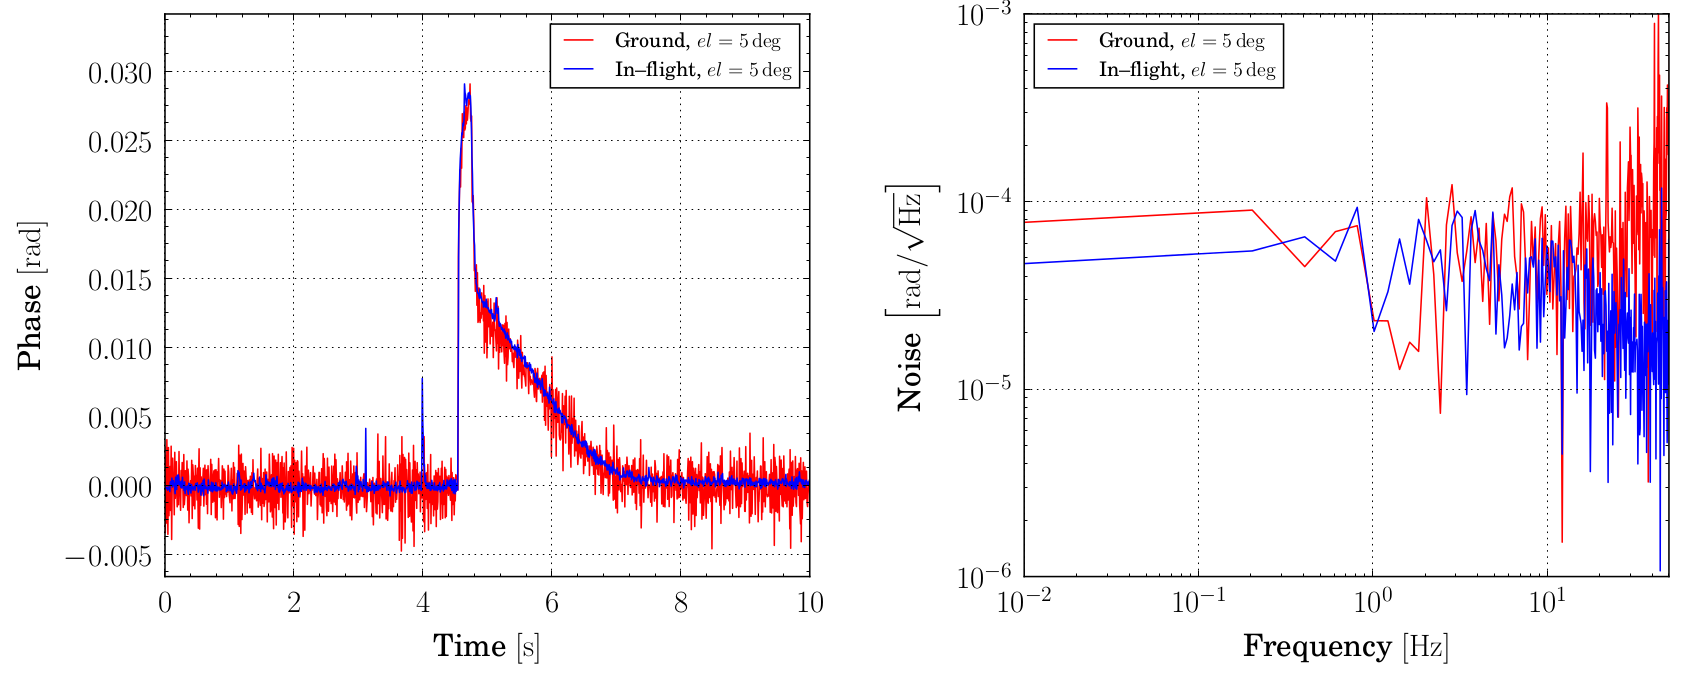
\includegraphics[width=\textwidth]{figures/intro/olimpo_cal_lamp}
\caption[~A cal lamp chop and PSD from the 2018 OLIMPO balloon flight.]{Data from a single detector taken during the 2018 OLIMPO balloon flight. The left frame shows the timestream of a cal lamp chop, taken on the ground (red) and in flight (blue). The right frame is the noise PSD for the same channel, on the ground (red) and in-flight (blue). The noise is lower in-flight by a factor of $\sim$2.5, due to lower thermal loading on the detectors. Image is from \citet{masi2019kinetic}.}
\label{fig:olimpo cal lamp}
\end{figure}

\vspace{5mm}

\textit{TolTEC}: TolTEC \citep{toltec} is a mm-wave camera which will be a facility instrument on the LMT, with first-light planned for 2019. Its camera is based on $\sim$7,000 dual-polarization sensitive trilayer TiN/Ti/TiN horn-coupled LEKIDs, similar to those used in BLAST-TNG, distributed between three bands centered at 2, 1.4, and 1.11~mm (50, 220, and 280~GHz) \citep{austermann2018millimeter}. The readout uses the ROACH2 firmware, software and IF electronics which have been developed for BLAST-TNG ($\sim$13 readout slices, versus the 5 used for BLAST-TNG). When coupled to the 50~m aperture of the LMT, TolTEC will have unprecedented spatial resolution in the mm-wave band (9.5$\arcsec$, 6.3$\arcsec$ and 5$\arcsec$). This will enable it to produce several unique data sets.

Soon after first-light, the TolTEC collaboration will conduct Four Public Legacy Surveys which will be made freely accessible to the public after $\sim$1--2~years. Some of first science surveys that are planned for TolTEC include\footnote{\url{http://toltec.astro.umass.edu/science}}:

\begin{itemize}[nosep]
  \item 100~deg$^{2}$ Large Scale Structure Survey
  \item 1~deg$^{2}$ confusion limited Ultra-Deep Galaxy Survey
  \item 90~deg$^{2}$ Clouds-to-Cores Legacy Survey
  \item Legacy Surveys of Nearby Galaxies
  \item The Cluster Cosmology Survey
  \item Magnetic Fields and Star Formation
  \item The Interrogation of Comets
\end{itemize}

\vspace{5mm}

\textit{Mexico-UK Submillimeter Camera for Astronomy (MUSCAT)}: MUSCAT \cite{brien2018muscat} is a LEKID camera which will be installed at the LMT along with TolTEC. It is based on four sub-arrays of horn-coupled LEKIDs (1,600 in total) which are cooled to 100~mK, and will observe in a single band centered at 1.1~mm. MUSCAT utilizes the BLAST-TNG ROACH2 firmware and IF electronics.

\vspace{5mm}

\textit{SuperSpec}: SuperSpec (\citet{superspec};\citet{wheeler2018superspec}) is an on-chip filter-bank spectrometer based on antenna-coupled TiN KIDs which will have its first on-sky engineering run at the LMT in 2019. It will perform moderate resolution (R $\sim$ 300) spectroscopy over 190--310 GHz (1.57--0.98~mm) using 300 channels. SuperSpec will measure redshifted line emission (e.g., [CII]) in submillimeter galaxies (SMGs) at cosmological redshift $z$ of 5--9, as well as CO emission in galaxies at lower $z$.

The SuperSpec camera incorporates the ROACH2 electronics, firmware and software developed for the BLAST-TNG readout. Figure~\ref{fig:readout noise comp} \citep{mcgeehan2018low} shows a comparison between the fractional frequency noise \gls{Sxx} of the system measured at a base temperature of 210~mK using the SuperSpec ROACH2 system and a Vector Network Analyzer (VNA) for tone combs consisting of 1 (blue and green) and 50 (red and pink) channels. The noise power spectral densities (PSDs) are shown for timestreams which correspond to the on and off-resonance states (see Chapter~\ref{blast_data}). Horizontal lines represent the expected photon-noise at the LMT sight. The system noise (including the LNA, readout, and detectors) which is measured with the ROACH2 system is comparable to that which is measured using VNA, for both the single and multitone combs.

\begin{figure}[!htbp]
\centering
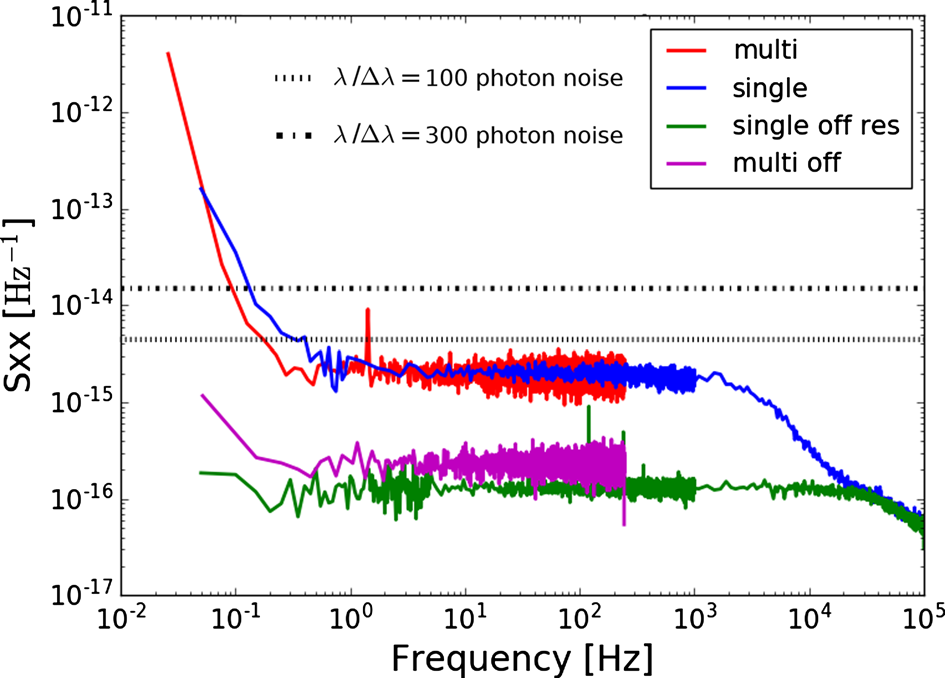
\includegraphics[width=\textwidth]{figures/intro/superspec_noisecomp}
\caption[~Comparison of the fractional frequency noise measured using the SuperSpec ROACH2 system and a VNA for single and multitone combs.]{A comparison of the fractional frequency noise \gls{Sxx} measured using the SuperSpec ROACH2 system and a VNA for single and multitone combs. The horizontal lines represent the expected photon-noise at the LMT sight. The ROACH2 system noise is comparable to that of the VNA, for both the single and multitone combs. Image taken from \citet{mcgeehan2018low}.}
\label{fig:readout noise comp}
\end{figure}

\vspace{5mm}

\textit{Future Instruments}: In addition to the experiments listed above, two recently funded balloon-borne cameras will incorporate elements of the ASU LEKID readout, with added improvements to the firmware and electronics which are made possible by the advent of ultra-high bandwidth FPGA boards (see~\ref{conclusion}). These are: The Experiment for Cryogenic Large-aperture Intensity Mapping (EXCLAIM) \citep{switzer2017measuring}, and the Terahertz Imager (TIM/STARFIRE) \citep{aguirre2018starfire}.

\section{Dissertation Outline}

This dissertation is organized as follows:

\begin{itemize}
\item Chapter~\ref{kid_model} describes a parametric model of a LEKID which can be used to simulate the behavior of both dark and optically loaded pixels, as well as to fit measurements of actual LEKIDs.

\item Chapter~\ref{readout} introduces the ASU LEKID readout, and details the system requirements, the architecture of the firmware, software and electronics, and the verification of the DSP pipeline and noise performance.

\item Chapter~\ref{blast_data} describes the instrumental characterization of the BLAST-TNG receiver and detector arrays which was conducted during the instrument integration at NASA's Columbia Scientific Balloon Facility (CSBF) in summer, 2018, as well as during pre-flight testing at NASA's Long Duration Balloon site (LDB) near McMurdo Station, Antarctica, during November through January, 2018/2019. The parametric LEKID model presented in Chapter~\ref{kid_model} is applied to measured detector data in order to understand various characteristics of the detector arrays and the instrument as a whole. Chapter

\item Chapter~\ref{carina} presents an original data analysis of the B-field morphology in the Carina Nebula Complex (CNC, NGC 3372), using a map of the region taken during the BLASTPol 2012 flight. In that analysis, we present what are possibly the first estimates of the strength of the plane-of-the-sky B-field (\gls{Bpos}) over the inner $\sim$1.25~deg$^{2}$ of the CNC.

\item Chapter~\ref{galaxies} presents a target selection survey of five nearby external galaxies which will be mapped during the 2019/2020 BLAST-TNG flight.

\item Chapter~\ref{mcp} contains an operator's manual for the $C$-based BLAST-TNG detector readout flight software, which includes a description of the in-flight detector readout strategy.

\item Chapter~\ref{conclusion} presents conclusions, with a discussion of how the technological landscape has evolved since this work began, and how it can benefit from recent developments in the area of high speed DSP.

\end{itemize}
